\chapter{Additional Figures and Tables}
\label{chap:app1}

\textbf{TBD}

\begin{table}[H]
    \small
    \setlength{\tabcolsep}{8pt}
    \renewcommand{\arraystretch}{1.3}
    \centering
        \caption[Normality Test - Shapiro--Wilk]{Normality Test - Shapiro--Wilk}\label{tab:normalitytest}
        \begin{tabular}{rrrr}
    \toprule
    \textbf{Feature} & \textbf{Shapiro-Wilk} & \textbf{Significance} & \textbf{Result}\\
    \midrule
    \hline
    LOAN & 0.8519 & *** & Not normally distributed \\ 
    MORTDUE & 0.8802 & *** & Not normally distributed \\ 
    VALUE & 0.81 & *** & Not normally distributed \\ 
    YOJ & 0.9078 & *** & Not normally distributed \\ 
    DEROG & 0.336 & *** & Not normally distributed \\ 
    DELINQ & 0.4578 & *** & Not normally distributed \\ 
    CLAGE & 0.9346 & *** & Not normally distributed \\ 
    NINQ & 0.6909 & *** & Not normally distributed \\ 
    CLNO & 0.9665 & *** & Not normally distributed \\ 
    DEBTINC & 0.8272 & *** & Not normally distributed \\
    \hline
    \bottomrule
    \end{tabular}
    \vspace{0.35em}

        \centering{\begin{source}Author's results in Python\end{source}}\vspace{-1em}
\end{table}


\begin{figure}[H]
    \centering
    \caption{WoE Bins Distribution}\vspace{0.5em}
    \label{fig:woedist}
    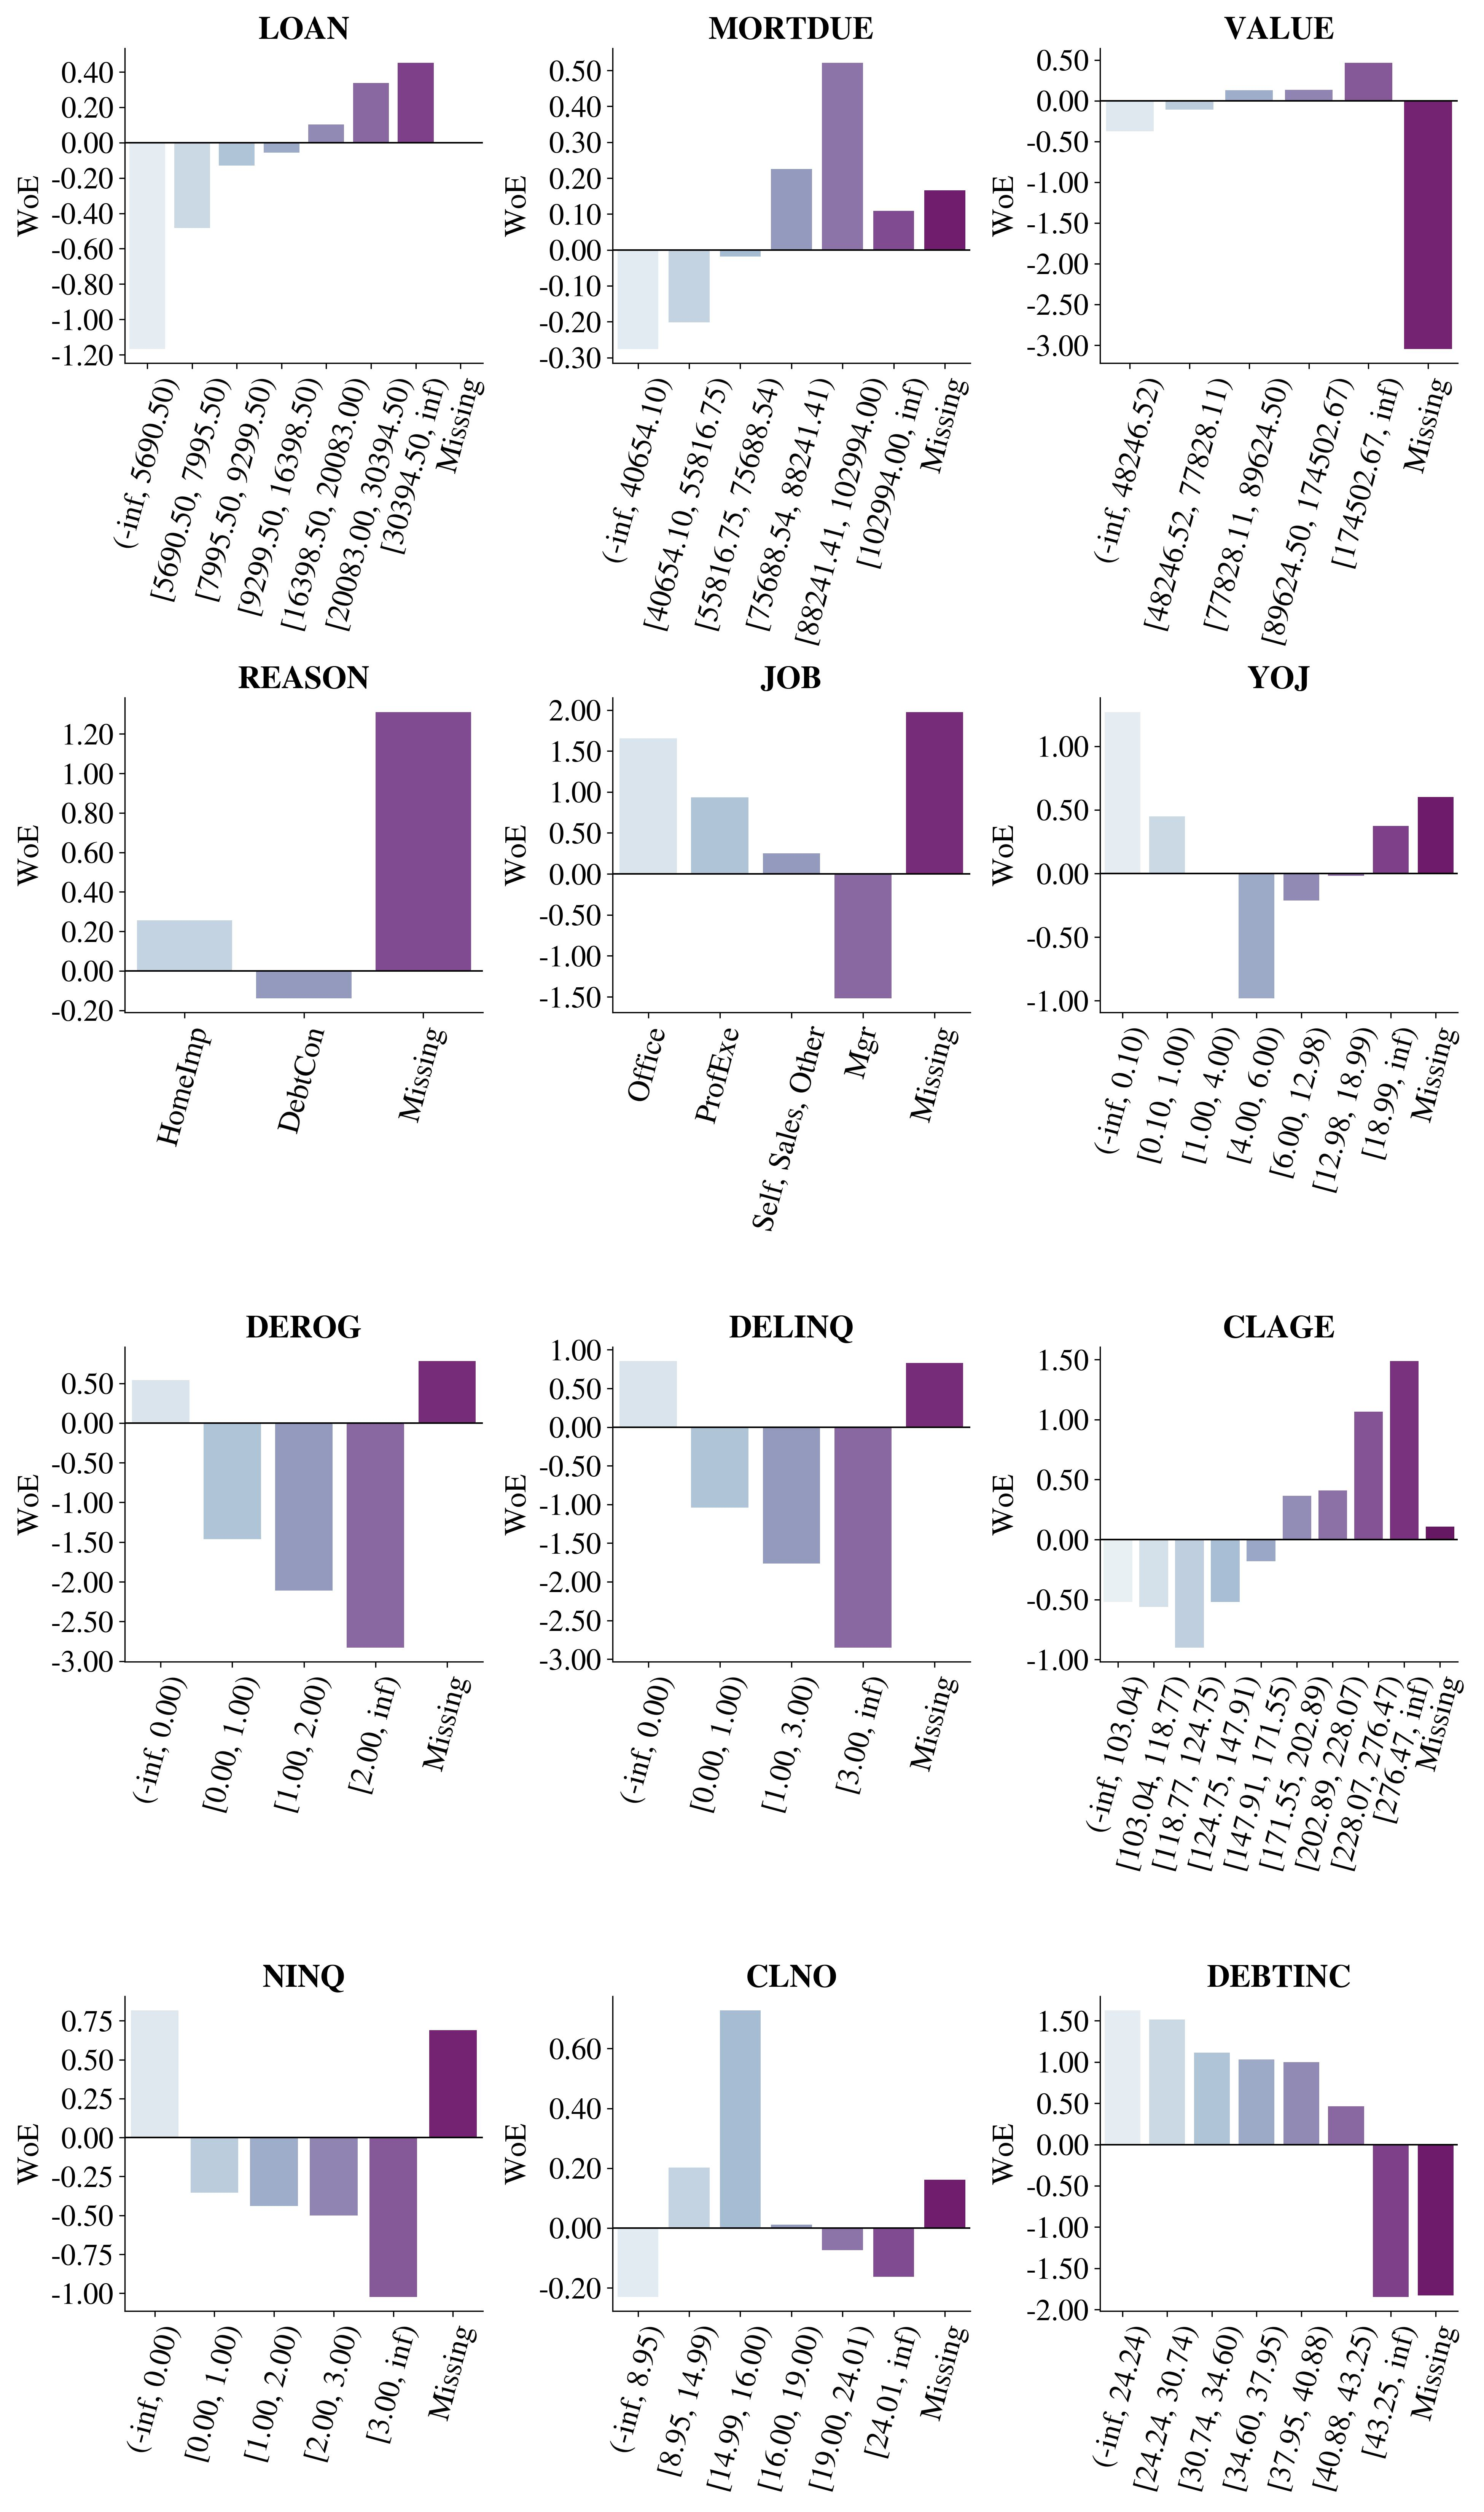
\includegraphics[width=140mm]{Figures/WoE_Distribution.jpg}
    
    \centering{\begin{source}Author's results in Python\end{source}}\vspace{-1em}
\end{figure}


